%二段組tex
%--------------------------------------------------------
\documentclass[twocolumn,10pt]{jarticle}
%----------------------------------------
%パッケージ
%----------------------------------------
\usepackage[top=20truemm,bottom=20truemm,left=20truemm,right=20truemm]{geometry}
\usepackage{amsmath,amssymb}
\usepackage{eucal}
\usepackage{bm}
\usepackage{ascmac}
\usepackage{pifont}
\usepackage{multirow}
\usepackage{enumerate}
\usepackage{cases}
\usepackage{url}
\usepackage[caption=false]{subfig}
\usepackage[ruled,vlined]{algorithm2e}
\usepackage{setspace}
\DeclareRelationFont{JY1}{mc}{it}{}{OT1}{cmr}{it}{}
\DeclareRelationFont{JT1}{mc}{it}{}{OT1}{cmr}{it}{}
\DeclareFontShape{JY1}{mc}{m}{it}{<5> <6> <7> <8> <9> <10> sgen*min
    <10.95><12><14.4><17.28><20.74><24.88> min10
    <-> min10}{}
\DeclareFontShape{JT1}{mc}{m}{it}{<5> <6> <7> <8> <9> <10> sgen*tmin
    <10.95><12><14.4><17.28><20.74><24.88> tmin10
    <-> tmin10}{}
\DeclareRelationFont{JY1}{mc}{sl}{}{OT1}{cmr}{sl}{}
\DeclareRelationFont{JT1}{mc}{sl}{}{OT1}{cmr}{sl}{}
\DeclareFontShape{JY1}{mc}{m}{sl}{<5> <6> <7> <8> <9> <10> sgen*min
    <10.95><12><14.4><17.28><20.74><24.88> min10
    <-> min10}{}
\DeclareFontShape{JT1}{mc}{m}{sl}{<5> <6> <7> <8> <9> <10> sgen*tmin
    <10.95><12><14.4><17.28><20.74><24.88> tmin10
    <-> tmin10}{}
\DeclareRelationFont{JY1}{mc}{sc}{}{OT1}{cmr}{sc}{}
\DeclareRelationFont{JT1}{mc}{sc}{}{OT1}{cmr}{sc}{}
\DeclareFontShape{JY1}{mc}{m}{sc}{<5> <6> <7> <8> <9> <10> sgen*min
    <10.95><12><14.4><17.28><20.74><24.88> min10
    <-> min10}{}
\DeclareFontShape{JT1}{mc}{m}{sc}{<5> <6> <7> <8> <9> <10> sgen*tmin
    <10.95><12><14.4><17.28><20.74><24.88> tmin10
    <-> tmin10}{}
\DeclareRelationFont{JY1}{gt}{it}{}{OT1}{cmbx}{it}{}
\DeclareRelationFont{JT1}{gt}{it}{}{OT1}{cmbx}{it}{}
\DeclareFontShape{JY1}{mc}{bx}{it}{<5> <6> <7> <8> <9> <10> sgen*goth
    <10.95><12><14.4><17.28><20.74><24.88> goth10
    <-> goth10}{}
\DeclareFontShape{JT1}{mc}{bx}{it}{<5> <6> <7> <8> <9> <10> sgen*tgoth
    <10.95><12><14.4><17.28><20.74><24.88> tgoth10
    <-> tgoth10}{}
\DeclareRelationFont{JY1}{gt}{sl}{}{OT1}{cmbx}{sl}{}
\DeclareRelationFont{JT1}{gt}{sl}{}{OT1}{cmbx}{sl}{}
\DeclareFontShape{JY1}{mc}{bx}{sl}{<5> <6> <7> <8> <9> <10> sgen*goth
    <10.95><12><14.4><17.28><20.74><24.88> goth10
    <-> goth10}{}
\DeclareFontShape{JT1}{mc}{bx}{sl}{<5> <6> <7> <8> <9> <10> sgen*tgoth
    <10.95><12><14.4><17.28><20.74><24.88> tgoth10
    <-> tgoth10}{}
\DeclareRelationFont{JY1}{gt}{sc}{}{OT1}{cmbx}{sc}{}
\DeclareRelationFont{JT1}{gt}{sc}{}{OT1}{cmbx}{sc}{}
\DeclareFontShape{JY1}{mc}{bx}{sc}{<5> <6> <7> <8> <9> <10> sgen*goth
    <10.95><12><14.4><17.28><20.74><24.88> goth10
    <-> goth10}{}
\DeclareFontShape{JT1}{mc}{bx}{sc}{<5> <6> <7> <8> <9> <10> sgen*tgoth
    <10.95><12><14.4><17.28><20.74><24.88> tgoth10
    <-> tgoth10}{}
\DeclareRelationFont{JY1}{gt}{it}{}{OT1}{cmr}{it}{}
\DeclareRelationFont{JT1}{gt}{it}{}{OT1}{cmr}{it}{}
\DeclareFontShape{JY1}{gt}{m}{it}{<5> <6> <7> <8> <9> <10> sgen*goth
    <10.95><12><14.4><17.28><20.74><24.88> goth10
    <-> goth10}{}
\DeclareFontShape{JT1}{gt}{m}{it}{<5> <6> <7> <8> <9> <10> sgen*tgoth
    <10.95><12><14.4><17.28><20.74><24.88> tgoth10
    <-> tgoth10}{}
\endinput
%%%% end of jdummy.def
\usepackage{here}
\usepackage[dvipdfmx]{graphicx}
\usepackage[dvipdfmx]{color}
%----------------------------------------
%各設定
%----------------------------------------
\setlength{\columnsep}{3zw}
\makeatletter
\newcommand{\figcaption}[1]{\def\@captype{figure}\caption{#1}}
\newcommand{\tblcaption}[1]{\def\@captype{table}\caption{#1}}
\renewcommand{\thefigure}{\thesection.\arabic{figure}}
\@addtoreset{figure}{section}
\renewcommand{\thetable}{\thesection.\arabic{table}}
\@addtoreset{table}{section}
\renewcommand{\theequation}{\arabic{section}.\arabic{equation}}
\@addtoreset{equation}{section}
\makeatother
\renewcommand{\figurename}{Fig.}
\renewcommand{\tablename}{Table}
%----------------------------------------

%----------------------------------------
\title{\vspace{-20truemm}
{\normalsize \rightline{平成29年\ 5月\ 20日}}  %日付
{\large 知的システム構成特論\\} %科目名
{\large Data Structures and Algorithms, %本の名前
Chapter 12 (pp.379-410)\\} %章番号とページ
メモリ管理 %タイトル
\date{}
\vspace{-2truemm}}
%----------------------------------------
\author{西田研究室 17344299 工大 太郎} %番号氏名
%--------------------------------------------------------
\begin{document}
\twocolumn[\maketitle]
%--------------------------------------------------------
%1章
%--------------------------------------------------------
\section{\TeX について}
%--------------------------------------------------------
TeXはスタンフォード大学教授(数学)D.E.Knuth(19388~)による文書整形システムです.TeXは大抵「テフ」と読まれています\cite{text_nn}.($\leftarrow$ 参考文献の引用) TeXはワープロのたぐいと言えますが,より正しくは,1つのプログラム言語に近いものです.利用者によるマクロ命令によって機能を拡張することができます.今までは研究者の間でUNIX環境での稼働が一般的でしたが,今日では,個人がMacintoshOSやWindows9Xをインストールしたパーソナルコンピュータ上でTeXを動かすことが可能です.ネットワークで配布されているパッケージもありますが,最近では,安価にCD-ROMの形態で書籍に付録されているものもあり,ある程度の文法の理解は必要ですが,文書作成の種類や目的によっては,とても重宝なツールと言えます.
\\(本当は敬語はだめ!!)
%--------------------------------------------------------
%2章
%--------------------------------------------------------
\section{\TeX について}
%--------------------------------------------------------
TeXはスタンフォード大学教授(数学)D.E.Knuth(19388~)による文書整形システムです.TeXは大抵「テフ」と読まれています.TeXはワープロのたぐいと言えますが,より正しくは,1つのプログラム言語に近いものです.なんとなく $f(x)$ の式を (\ref{eq:simple_z})~式に示す.
%-------------------------------
\begin{equation}
\mbox{\boldmath{$z$}} = f(x)\mbox{\boldmath{$a$}}
%ベクトルaは\mbox{\boldmath{$a$} と書く.
\label{eq:simple_z}
\end{equation}
%-------------------------------
なんとなく図を {\bf Fig.~\ref{fig:grasp_evaluator}} に示す.今までは研究者の間でUNIX環境での稼働が一般的でしたが,今日では,個人がOSをインストールしたパーソナルコンピュータ上でTeXを動かすことが可能です.
%-------------------------------
\vspace{10mm}
\begin{figure}[H]
\centering
  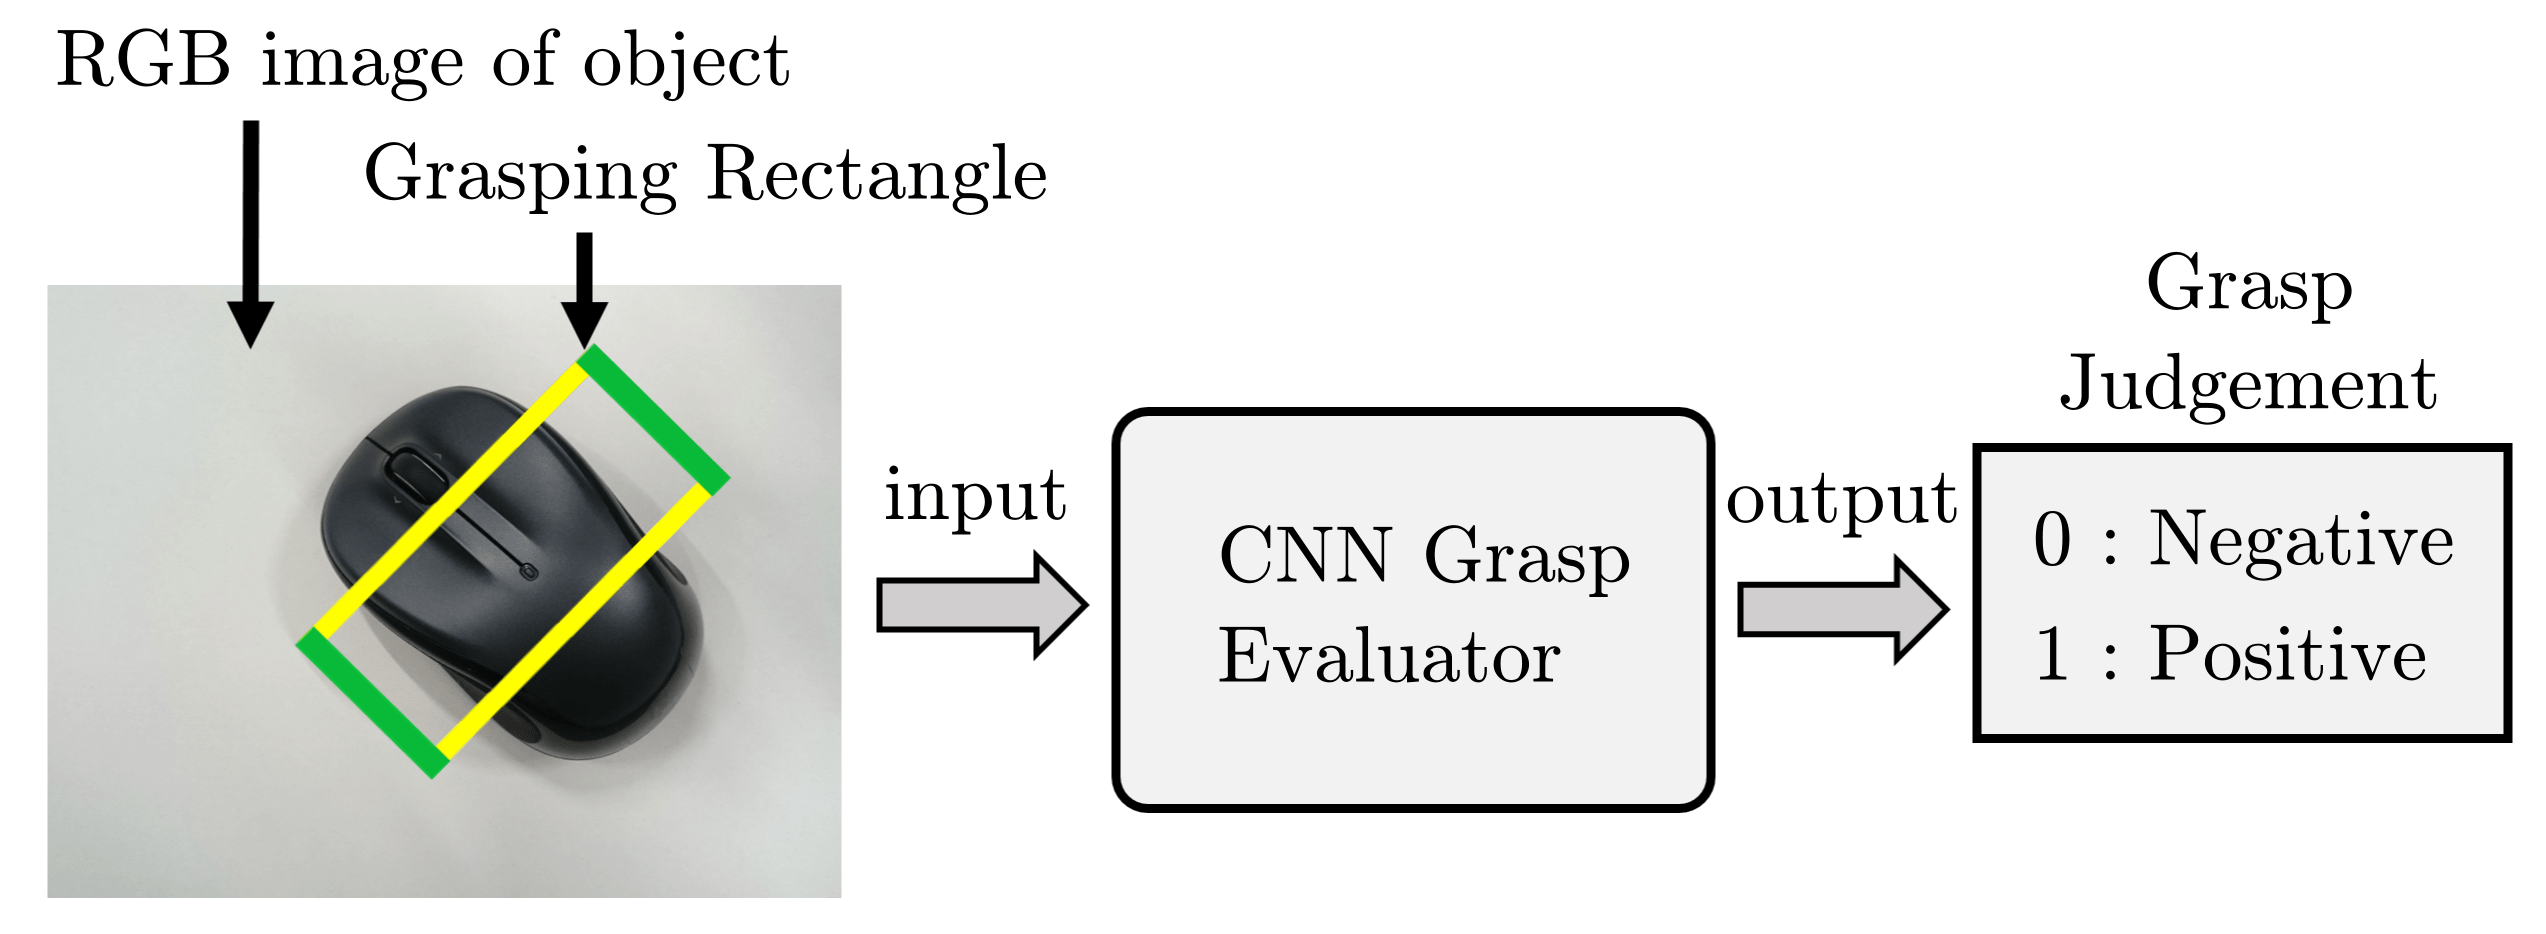
\includegraphics[scale=0.08]{../figures/evaluator.png}
\caption{Grasp evaluator.}
\label{fig:grasp_evaluator}
\end{figure}
%-------------------------------
%--------------------------------------------------------
%3章
%--------------------------------------------------------
\section{\TeX について}
TeXはスタンフォード大学教授(数学)D.E.Knuth(19388~)による文書整形システムです.TeXは大抵「テフ」と読まれています.TeXはワープロのたぐいと言えますが,より正しくは,1つのプログラム言語に近いものです.なんとなくアルゴリズムを {\bf Algorithm~\ref{alg:grasp}} に示す.
%-------------------------------
\begin{spacing}{0.99}
\begin{algorithm}[htbp]
\caption{Random Grasp Planning}
\label{alg:grasp}
\nl Load learned CNN model : ${\rm CNN}(\mbox{\boldmath{$Image$}},\mbox{\boldmath{$Rectangle$}})$\\
\nl Take an RGB color picture of the object : $\mbox{\boldmath{$I$}}_{\rm m}$\\
\nl\While{${\rm true}$}{
\nl Generate grasp rectangle randomly : $\mbox{\boldmath{$R$}}_{\rm rand}$\\
\nl $N_{\rm out} \longleftarrow {\rm CNN}(\mbox{\boldmath{$I$}}_{\rm m},\mbox{\boldmath{$R$}}_{\rm rand})$\\
\nl\If{$N_{\rm out} = {\rm true}$}{
\nl ${\rm {\bf break}}$\\}}
\nl $\mbox{\boldmath{$R$}}_{\rm out} \longleftarrow \mbox{\boldmath{$R$}}_{\rm rand}$\\
\end{algorithm}
\end{spacing}
\vspace{-10mm}
%-------------------------------
%--------------------------------------------------------
%4章
%--------------------------------------------------------
\section{\TeX について}
%--------------------------------------------------------
TeXはスタンフォード大学教授(数学)D.E.Knuth(19388~)による文書整形システムです.TeXは大抵「テフ」と読まれています.TeXはワープロのたぐいと言えますが,より正しくは,1つのプログラム言語に近いものです.利用者によるマクロ命令によって機能を拡張することができます.今までは研究者の間でUNIX環境での稼働が一般的でしたが,今日では,個人がMacintoshOSやWindows9Xをインストールしたパーソナルコンピュータ上でTeXを動かすことが可能です.なんとなく表を {\bf Table~\ref{tb:gyudon}} に示す.
%-------------------------------
\begin{table}[H]
\caption{Results of grasp planning.}
\centering
\vspace{4mm}
  \begin{tabular}{|l|c|r||r|} \hline
    メニュー & サイズ & 値段 & カロリー \\ \hline \hline
    牛丼 & 並盛 & 500円 & 600 kcal \\
    牛丼 & 大盛 & 1,000円 & 800 kcal \\
    牛丼 & 特盛 & 1,500円 & 1,000 kcal \\ \hline
    牛皿 & 並盛 & 300円 & 250 kcal \\
    牛皿 & 大盛 & 700円 & 300 kcal \\
    牛皿 & 特盛 & 1,000円 & 350 kcal \\ \hline
  \end{tabular}
\label{tb:gyudon}
\end{table}
%--------------------------------------------------------
%5章
%--------------------------------------------------------
\section{\TeX について}
%--------------------------------------------------------
TeXはスタンフォード大学教授(数学)D.E.Knuth(19388~)による文書整形システムです.TeXは大抵「テフ」と読まれています.TeXはワープロのたぐいと言えますが,より正しくは,1つのプログラム言語に近いものです.利用者によるマクロ命令によって機能を拡張することができます.今までは研究者の間でUNIX環境での稼働が一般的でしたが,今日では,個人がMacintoshOSやWindows9Xをインストールしたパーソナルコンピュータ上でTeXを動かすことが可能です.ネットワークで配布されているパッケージもありますが,最近では,安価にCD-ROMの形態で書籍に付録されているものもあり,ある程度の文法の理解は必要ですが,文書作成の種類や目的によっては,とても重宝なツールと言えます.……以下続く……
%--------------------------------------------------------
%6章
%--------------------------------------------------------
\section{\TeX について}
%--------------------------------------------------------
TeXはスタンフォード大学教授(数学)D.E.Knuth(19388~)による文書整形システムです.TeXは大抵「テフ」と読まれています.TeXはワープロのたぐいと言えますが,より正しくは,1つのプログラム言語に近いものです.利用者によるマクロ命令によって機能を拡張することができます.今までは研究者の間でUNIX環境での稼働が一般的でしたが,今日では,個人がMacintoshOSやWindows9Xをインストールしたパーソナルコンピュータ上でTeXを動かすことが可能です.ネットワークで配布されているパッケージもありますが,最近では,安価にCD-ROMの形態で書籍に付録されているものもあり,ある程度の文法の理解は必要ですが,文書作成の種類や目的によっては,とても重宝なツールと言えます.……以下続く……
%--------------------------------------------------------
%7章
%--------------------------------------------------------
\section{\TeX について}
%--------------------------------------------------------
TeXはスタンフォード大学教授(数学)D.E.Knuth(19388~)による文書整形システムです.TeXは大抵「テフ」と読まれています.TeXはワープロのたぐいと言えますが,より正しくは,1つのプログラム言語に近いものです.利用者によるマクロ命令によって機能を拡張することができます.今までは研究者の間でUNIX環境での稼働が一般的でしたが,今日では,個人がMacintoshOSやWindows9Xをインストールしたパーソナルコンピュータ上でTeXを動かすことが可能です.ネットワークで配布されているパッケージもありますが,最近では,安価にCD-ROMの形態で書籍に付録されているものもあり,ある程度の文法の理解は必要ですが,文書作成の種類や目的によっては,とても重宝なツールと言えます.……以下続く……
%--------------------------------------------------------
%8章
%--------------------------------------------------------
\section{\TeX について}
%--------------------------------------------------------
TeXはスタンフォード大学教授(数学)D.E.Knuth(19388~)による文書整形システムです.TeXは大抵「テフ」と読まれています.TeXはワープロのたぐいと言えますが,より正しくは,1つのプログラム言語に近いものです.利用者によるマクロ命令によって機能を拡張することができます.今までは研究者の間でUNIX環境での稼働が一般的でしたが,今日では,個人がMacintoshOSやWindows9Xをインストールしたパーソナルコンピュータ上でTeXを動かすことが可能です.ネットワークで配布されているパッケージもありますが,最近では,安価にCD-ROMの形態で書籍に付録されているものもあり,ある程度の文法の理解は必要です.
%--------------------------------------------------------
%9章
%--------------------------------------------------------
\section{\TeX について}
%--------------------------------------------------------
TeXはスタンフォード大学教授(数学)D.E.Knuth(19388~)による文書整形システムです.TeXは大抵「テフ」と読まれています.TeXはワープロのたぐいと言えますが,より正しくは,1つのプログラム言語に近いものです.利用者によるマクロ命令によって機能を拡張することができます.今までは研究者の間でUNIX環境での稼働が一般的でしたが,今日では,個人がMacintoshOSやWindows9Xをインストールしたパーソナルコンピュータ上でTeXを動かすことが可能です.
%-------------------------------
\begin{thebibliography}{99}
\addcontentsline{toc}{section}{参考文献}
%-------------------------------
\bibitem{text_nn} 岡谷貴之,『深層学習』(機械学習プロフェッショナルシリーズ),講談社, pp.7-33, pp.41-54, pp79-97, 2015.
%-------------------------------
\bibitem{IanLenz} Ian Lenz, Honglak Lee,
 and Ashutosh Saxena.
 ``Deep Learning for Detecting Robotic Grasps'',
 The International Journal of Robotics Research,
 34(4-5),pp.705-724, 2015.
%-------------------------------
\bibitem{PCL} PCL - Pint Cloud Library, accessed
 10 February 2017, $<$\url{http://www.pointclouds.org/}$>$
%-------------------------------
\end{thebibliography}
\end{document}
